\section{Ejercicios propuestos.}

\subsection{Ejercicio Propuesto 1}

Sea un estrato homogéneo e isótropo formado por arenas que tiene un
espesor de 5.2 m y coeficiente de permeabilidad
$k_x=k_y=k_z=1\cdot10^{-2}$ m/s. Debajo de él hay otro estrato
homogéneo e isótropo formado por arenas limosas con un espesor de 4
metros y con coeficiente de permeabilidad $k_x=k_y=k_z=5\cdot10^{-5}$
m/s. Bajo las arenas limosas hay un estrato de arcillas que se asume
son impermeables. Para reducir la filtración debida al primer estrato
se ha clavado una tablestaca (de longitud infinita en la dirección
perpendicular al plano del dibujo) que, por error de ejecución, sólo
ha penetrado 4.6 m. A la izquierda de la tablestaca (aguasarriba) se
ha acumulado una altura de 3 metros de agua y a la derecha (aguas
abajo) la escorrentía hace no haya acumulación de agua. Para el
problema así definido (ver Fig.~\ref{enu02}) y asumiendo un régimen
estacionario responde a la pregunta que te harán en clase.
\begin{figure}[!h]
  \begin{center}
    \includegraphics[width=0.75\textwidth]{./body/images/enu02}
  \end{center}
  \caption{Descripción del modelo}
  \label{enu02}
\end{figure}



\paragraph{NOTA:} Usa el mismo tipo de elementos que en el ejercicio resuelto y un tamaño global de malla de 1.4 metros.

\paragraph{AYUDA:} En este ejercicio hay dos materiales diferentes que
comparten una frontera común. Para reproducirlo en Abaqus sigue los
siguientes pasos:

\begin{itemize}
\item Crea una \textit{part} diferente para cada estrato y asígnales
  el material correspondiente. Cuando estés en el módulo
  \textbf{Property} y vayas a asignar una sección a una \textit{part}
  (comando \textbf{Assign Section}) recuerda no crear un \textit{set},
  tal como indica la Fig.~\ref{corr01} (es para evitar problemas en la
  operación \textbf{Merge} posterior).
  \begin{figure}[!h]
    \begin{center}
      
\includegraphics[width=0.75\textwidth]{./body/images/corr01.pdf}
    \end{center}
    \caption{\textit{Prompt} asociado a \textbf{Assign Section}}
    \label{corr01}
  \end{figure}
\item En el módulo \textbf{Assemble} ensambla un modelo con una copia
  dependiente de cada parte como indica la
  Fig.\ref{ayu01}. Posteriormente pulsa el comando \textbf{Translate
    Instance} (ver Fig.~\ref{ayu02}) hasta dejarlas en su posición
  definitiva (ver Fig.~\ref{ayu03}).
  \begin{figure}[!h]
    \centering
    \begin{subfigure}[!h]{0.95\textwidth}
      \includegraphics[width=\textwidth]{./body/images/ayu01}
      \caption{Posición inicial de las copias de las \textit{parts}}
      \label{ayu01}
    \end{subfigure}%
    
    % add desired spacing between images, e. g. ~, \quad, \qquad,
    % \hfill etc.
    % (or a blank line to force the subfigure onto a new line)
    \begin{subfigure}[!h]{0.15\textwidth}
      \includegraphics[width=\textwidth]{./body/images/ayu02.pdf}
      \caption{Comando \textbf{Translate Instance}}
      \label{ayu02}
    \end{subfigure}%
    \begin{subfigure}[!h]{0.82\textwidth}
      \includegraphics[width=\textwidth]{./body/images/ayu03}
      \caption{Posición final de las copias de las \textit{parts}}
      \label{ayu03}
    \end{subfigure}%
    \caption{Ensamblar un modelo con dos \textit{parts} I}
  \end{figure}

\item Finalmente buscamos crear una nueva \textit{part} como la unión
  de las dos anteriores pero conservando la frontera común entre
  ellas. Para hacerlo pulsa \textbf{Merge/Cut} (ver Fig.~\ref{ayu02r})
  asegurándote que activas la opción \textbf{Retain Boundary} (ver
  Fig.~\ref{ayu04}). Revisa que en el nodo de las
  \textit{Assembly/Instances} del \textbf{Model Tree} se ha creado la
  nueva copia (ver Fig.~\ref{ayu05})

  \begin{figure}[!h]
    \centering
    \begin{subfigure}[!h]{0.15\textwidth}
      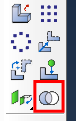
\includegraphics[width=\textwidth]{./body/images/ayu02r}
      \caption{Comando \textbf{Merge/Cut}}
      \label{ayu02r}
    \end{subfigure}%
    % add desired spacing between images, e. g. ~, \quad, \qquad,
    % \hfill etc.
    % (or a blank line to force the subfigure onto a new line)
    \begin{subfigure}[!h]{0.45\textwidth}
      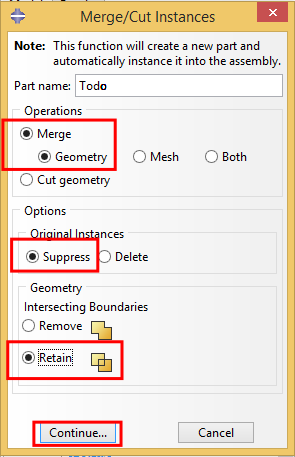
\includegraphics[width=\textwidth]{./body/images/ayu04.pdf}
      \caption{Cuadro de diálogo \textbf{Merge/Cut}}
      \label{ayu04}
    \end{subfigure}%
    \begin{subfigure}[!h]{0.20\textwidth}
      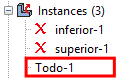
\includegraphics[width=\textwidth]{./body/images/ayu05}
      \caption{Copias creadas en el modelo}
      \label{ayu05}
    \end{subfigure}%
    \caption{Ensamblar un modelo con dos \textit{parts} II}
  \end{figure}
\item Recuerda que cuando vayas a mallar deber hacerlo sobre la nueva
  \textbf{Part} creada tal como indica la Fig.~\ref{ayu06}.
  \begin{figure}[!h]
    \centering
    \includegraphics[width=0.95\textwidth]{./body/images/ayu06}
    \caption{Mallado de la nueva \textit{part}}
    \label{ayu06}
  \end{figure}

\end{itemize}
\clearpage \newpage

\subsection{Ejercicio Propuesto 2}

Sea una presa cuya base tiene 27 metros construida en hormigón (que
asumiremos es impermeable) de longitud infinita en la dirección
perpendicular al plano del dibujo. Bajo la base hay un estrato
homogéneo e isótropo de arena limosa con una permeabilidad
$k_x=k_y=k_z=5\cdot10^{-5}$ m/s y un espesor de 15 m. Bajo este
estrato hay un paquete de arcillas que asumiremos son impermeables.

Se dispone, para evitar la filtración, de una pantalla de 5 metros de
altura en el extremo de aguas arriba de la presa y, para evitar la
subpresión, de un dren de escollera de 7 m de largo y 1 m de alto con
una permeabilidad de $k_x=k_y=k_z=1\cdot10^{-1}$ m/s.

Aguas arriba de la presa se acumula una altura de 10 metros de agua y
aguas abajo la escorrentía hace no haya acumulación de agua. Para el
problema así definido (ver Fig.~\ref{enu03}) y asumiendo un régimen
estacionario se pide:
\begin{enumerate}
\item Obtener el caudal de agua saliente aguas abajo (por unidad de
  longitud de la dirección $y$).
\item Obtener la resultante de la subpresión (fuerza vertical) en la
  recta DE por unidad de longitud de la dirección $y$.
\end{enumerate}



\begin{figure}[!h]
  \begin{center}
    \includegraphics[width=0.95\textwidth]{./body/images/enu03}
  \end{center}
  \caption{Descripción del modelo}
  \label{enu03}
\end{figure}

\paragraph{NOTA:} Usa el mismo tipo de elementos que en el ejercicio
resuelto y un tamaño global de malla de 2.5 metros. La solución a la
pregunta 1 es 1.942e-4 m$^3$/s por metro en la dirección $y$. La
solución a la pregunta 2 es 699.8 kN por metro en la dirección $y$.

\paragraph{AYUDA:} En este ejercicio hay dos materiales diferentes que
comparten una frontera común. Para reproducir ésto en Abaqus sigue los
pasos indicados en la ayuda del Ejercicio 1.
\hspace{20mm}\hrulefill$\star$\hrulefill\hspace{20mm}

\clearpage \newpage
\subsection{Ejercicio Propuesto 3}


Sea una presa construida en hormigón (que consideraremos impermeable)
de longitud infinita en la dirección perpendicular al plano del
dibujo. Bajo la base hay un estrato formado por dos materiales
homogéneos e isótropos de arena limosa y bajo ese estrato hay un
paquete de arcillas que asumiremos son impermeables.  Se construye,
para reducir la filtración, una pantalla en el extremo de aguas arriba
de la presa (considerar la pantalla de espesor 0.05 m.).  La geometría
y las propiedades de permeabilidad de los materiales se describen en
la Fig.~\ref{enup01nn}. Asumiremos que las fronteras verticales del
estrato en los extremos están tan alejadas de la presa como para
considerarlas impermeables.  En el punto D queremos simular el efecto
de una bomba que extrae un caudal de 0.0001 m$^3$/s por metro lineal
en la dirección $z$. Para hacerlo, consulta en la ayuda de Abaqus el
comando \textbf{Concentrated heat flux} (piensa el signo que debes
poner para simular que estamos extrayendo caudal).  \vspace{-2mm}
\begin{figure}[!h]
  \centering
  \includegraphics[width=0.99\linewidth]{./body/images/enup01}
  \caption{Descripción del problema}
  \label{enup01nn}
\end{figure}

Responde las preguntas que vienen a continuación con las siguientes
consideraciones:
\begin{itemize}
\item usa al definir la malla elementos cuadriláteros, técnica de
  mallado \textit{Free}, con tamaño global de malla 1.8 metros e
  interpolación cuadrática (elemento \textit{DC2D8}). No subdividas
  las parts para obtener una malla más regular.
\item considera el fluido es agua dulce con densidad $\rho_w=1000$
  kg/m$^3$ y que la aceleración de la gravedad vale $g=9.81$ m/s$^2$.
\item Para facilitar el cálculo de la subpresión, considera que el
  origen de las alturas (\textit{z=0} m.) está en la base de la presa
  DF.
\end{itemize}

Para el problema así definido calcula el caudal saliente en la recta
GH por unidad de metro en la dirección $z$ (la solución es 0.00108
m$^3$/s/ml) y la fuerza vertical de subpresion bajo la presa (la
solución es 613.37 kN/ml).  \vspace{3mm}

\hspace{20mm}\hrulefill$\star$\hrulefill\hspace{20mm}

\clearpage \newpage
\subsection{Ejercicio Propuesto 4}

Sea un terreno en el que hemos clavado las dos tablestacas de la figura
(que consideraremos impermeables y de espesor 0.05 m) de longitud infinita
en la dirección $z$. Este estrato está formado por tres materiales homogéneos
e isótropos de arena limosa.
Bajo ese estrato hay un paquete de arcillas que asumiremos son
impermeables.  La geometría y las propiedades de permeabilidad de
los materiales se describen en la Fig.~\ref{enup04}.
A la izquierda de la tablestaca 1  se acumula un volumen de agua
con una altura sobre el punto H de 15 m.~constante. Entre las tablestacas 1 y 2
construimos una placa de hormigón que hace impermeable el contorno CD. A la derecha de la tablestaca 2 dispone una red de inyectores que aplican flujo entrante de valor $q=10^{-3}$ m$^3$/m$^2$/s en el contorno EF. Finalmente en el tramo FG la escorrentía hace que no se
acumule agua por encima del terreno. Asumiremos que las fronteras
verticales del estrato en los extremos están tan alejadas de las tablestacas
como para considerarlas impermeables.  \vspace{-2mm}
\begin{figure}[!h]
  \centering
  \includegraphics[width=1.0\linewidth]{./body/images/enup04}
  \caption{Descripción del problema}
  \label{enup04}
\end{figure}

Usa las siguientes
consideraciones (al ser un problema plano, tomaremos un espesor unidad
y los valores de caudal y fuerza serán por por metro en la dirección $z$):
\begin{itemize}
\item Usa al definir la malla elementos cuadriláteros, técnica de
  mallado \textit{Free}, con tamaño global de malla 1.3 metros e
  interpolación lineal (el tipo de elemento deberá ser \textit{DC2D4}). No subdividas las
  parts para obtener una malla más regular.
\item Considera el fluido es agua dulce con densidad $\rho_w=1000$
  kg/m$^3$ y que la aceleración de la gravedad vale $g=9.81$ m/s$^2$.
\item Las recta que separa los materiales 1 y 3 es vertical.
\item \textbf{Utiliza como origen de las alturas geométricas la recta horizontal
    que pasa por H.}
\end{itemize}

Para el problema así descrito calcula la fuerza vertical de subpresión bajo el bloque CD (1454.8 kN), la presión de poro del fluido en el punto A (170.6 kPa), la altura total del punto B (2.67 m), el módulo del vector flujo en el centroide del elemento E1 ($9.62\cdot 10^{-5}$ m$^3$/m$^2$/s) y el caudal que atraviesa la recta BI (0.00275 m$^3$/s) .